\chapter{評価実験}

\section{検証の目的}
本研究では，
第3章で提案した
髭密度を考慮した皮膚表面下散乱モデルの妥当性を検証することを目的とする。
提案手法は，
髭一本一本の幾何構造を直接扱うのではなく，
髭の分布を髭密度というスカラー量として近似し，
この密度に基づいて皮膚モデルと髭モデルを混合する点に特徴がある。

皮膚表面下散乱に対する髭の影響は，
髭自身が形成する遮蔽や影，
毛の太さや深さ，
配置のばらつきなど，
多くの要因が複雑に関与する現象である。
そのため，
髭を幾何構造として忠実に扱う場合，
計算コストが高くなるだけでなく，
得られる結果が
必ずしも安定した挙動を示すとは限らない。

本研究では，
このような複雑な要因をすべて厳密にモデル化するのではなく，
髭の分布を密度という抽象化された量として扱うことで，
表面下散乱特性を
安定かつ連続的に制御することを目指している。
したがって，
提案モデルの妥当性を評価する上で重要なのは，
幾何的な髭モデルを正確に再現できているかどうかではなく，
この抽象化が
設計意図どおりの振る舞いを
実際に生み出しているかを確認することである。

特に本章では，
髭密度の変化に応じて，
表面下散乱の空間的広がりや
放射束分布が，
不自然な不連続や破綻を生じることなく，
滑らかかつ安定して変化するかどうかを
モデルの妥当性の指標とする。

本章で検証する問いは，以下の2点である。
\begin{enumerate}
  \item 髭密度に基づく線形混合モデルが，
        表面下散乱分布を不自然に破綻させることなく，
        密度変化に対して連続的かつ安定に応答するか。
  \item 髭を幾何構造として直接扱った場合に観測される挙動と比較して，
        髭密度モデルが，
        表面下散乱特性を制御・評価するための
        実用的かつ妥当な抽象化として機能しているか。
\end{enumerate}

これらの問いに答えるため，
本章では定量的および定性的な評価を行う。
定量的評価では，
点光源入射時における
表面下散乱の空間分布を計測し，
入射点からの距離に対する減衰特性を比較する。
また，
定性的評価では，
髭密度を変化させたレンダリング画像を比較し，
見えの変化や
不自然なアーティファクトの有無を確認する。

\begin{enumerate}
  \item 髭密度を用いた線形混合が，
        表面下散乱分布を不自然に破綻させることなく，
        密度変化に対して連続に応答するか。
  \item 髭を幾何構造として直接扱う場合と比較して，
        髭密度による近似が，
        表面下散乱特性を評価する上で妥当な抽象化となっているか。
\end{enumerate}

これらの問いに答えるため，
本章では定量的および定性的な評価を行う。
定量的評価では，
点光源入射時における
表面下散乱の空間分布を計測し，
入射点からの距離に対する減衰特性を比較する。
また，
定性的評価では，
髭密度を変化させたレンダリング画像を比較し，
見えの変化やアーティファクトの有無を確認する。





\section{実験環境および共通設定}
本章における評価実験では，
提案した髭密度を考慮した皮膚表面下散乱モデルの挙動を
定量的に観測するため，
単純化した検証シーンを用いる。
レンダリングにはモンテカルロ法に基づくパストレーシングを用い，
表面下散乱の計算には
第3章で述べたBSSRDFモデルを組み込んだ。

定量評価では，
幾何形状や陰影の影響を排除し，
表面下散乱の空間的広がりのみを評価するため，
無限平面上に皮膚モデルを配置し，
点光源を垂直方向から入射させる構成を用いた。
この構成により，
入射点を基準とした距離依存の散乱特性を
明確に観測することが可能となる。

照明条件，反射モデルのパラメータ，
およびサンプル数は，
すべての実験条件において共通とし，
比較対象間で条件が一致するように設定した。
これにより，
観測される差異は
髭の有無やモデル化手法の違いに起因するものとして
解釈することができる。
実験シーンの概要を
図\ref{fig:exp_setup}に示す。
\begin{figure}[tb]
  \centering
  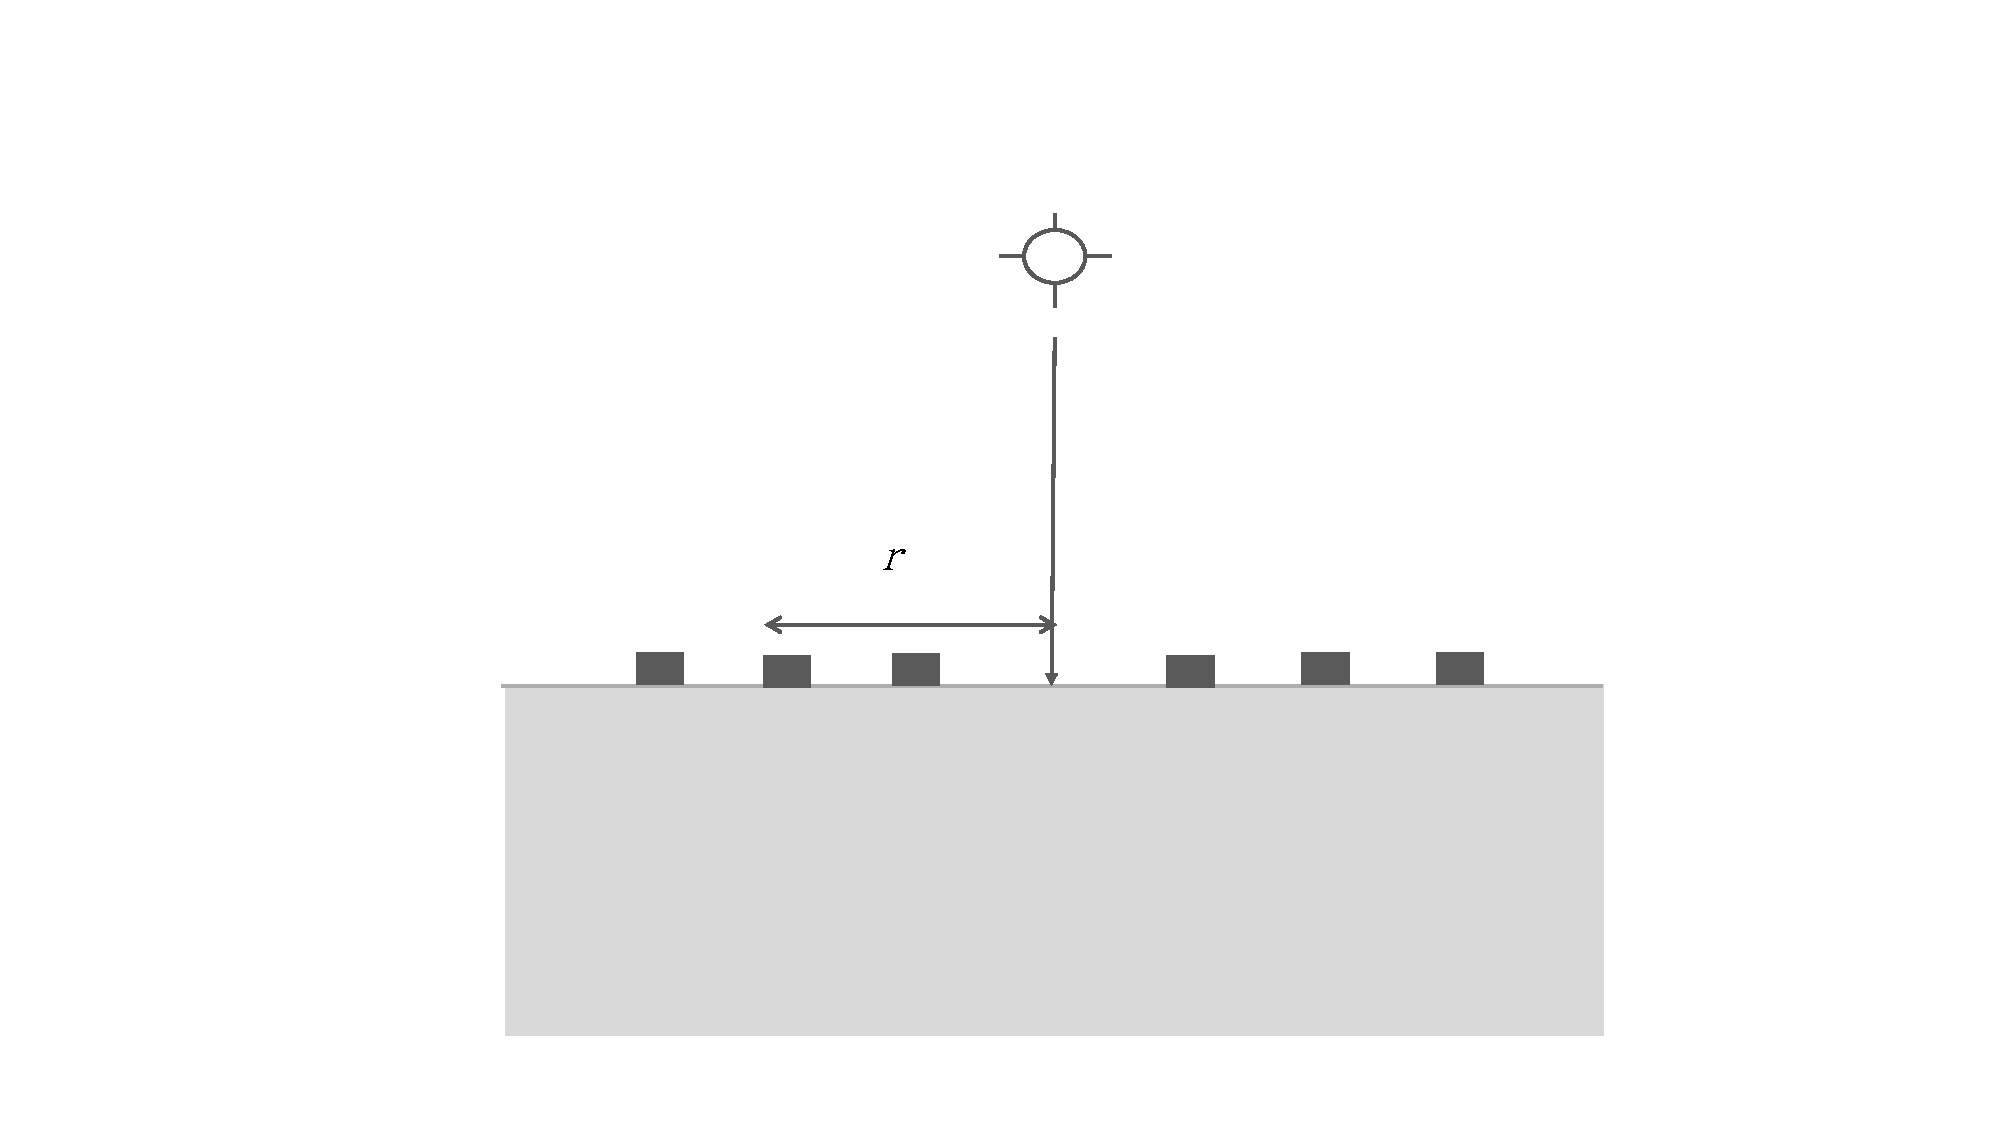
\includegraphics[width=0.8\linewidth]{figs/scene_setup.pdf}
  \caption{評価シーンの構成。無限平面上の入射点に点光源を垂直入射させ，
  入射点を中心とした半径 $r$ のリング上に配置した観測点で $R_d(r)$ を計測する。}
  \label{fig:exp_setup}
\end{figure}


\section{表面下散乱分布 $R_d(r)$ の計測}
\label{sec:rd_measure}
本節では，
表面下散乱の空間的な広がりを評価するために用いた
指標および計測方法について述べる。

\subsection{評価指標の定義}
\label{sec:rd_definition}
表面下散乱の広がりを評価する指標として，
入射点から距離 $r$ だけ離れた位置における
放射束分布 $R_d(r)$ を用いる。
$R_d(r)$ は，
点光源が皮膚表面に垂直入射した際に，
入射点を中心とする距離 $r$ の位置から
出射する放射束の分布を表す量であり，
表面下散乱による光の拡散特性を反映する。

本実験では，
表面上の同心円リングに沿って
複数の評価点を配置し，
各点における入射放射束を照度計によって計測した。
各距離 $r$ における $R_d(r)$ は，
円周方向にサンプリングした値の平均として算出する。
これにより，
角度方向のばらつきを抑え，
距離依存性に着目した評価が可能となる。

また，
分布形状の比較を容易にするため，
得られた $R_d(r)$ は
全距離にわたる面積積分が 1 となるよう正規化している。
この正規化により，
絶対的なエネルギー量ではなく，
距離方向の減衰特性そのものに着目した比較を行うことができる。

\subsection{計測シーンおよび手順}
\label{sec:rd_procedure}
計測は，
無限平面上に配置した皮膚モデルに対して，
点光源を垂直方向から入射させる構成で行った。
入射点を原点とし，
距離 $r$ に応じて
同心円状に評価点を配置することで，
幾何形状による影響を排除し，
表面下散乱の広がりのみを観測できるようにした。

各距離 $r$ において，
円周方向に複数点をサンプリングし，
それらの平均値を $R_d(r)$ として記録した。
評価点の配置および
計測手順の概念図は割愛する。


\section{幾何的髭モデルによる基礎検証}
\label{sec:geom_beard}
本節では，
提案する髭密度モデルの評価に先立ち，
髭を幾何構造として直接表現した場合の
表面下散乱分布の挙動を確認するための
基礎的な検証について述べる。

本検証では，
髭を円柱状の幾何構造としてモデル化し，
皮膚平面の内部に埋め込んだ。
円柱は皮膚表面に対して垂直に配置され，
その位置および本数は固定とした。
このような構成により，
髭を一本一本の幾何として忠実に扱った場合に，
表面下散乱分布 $R_d(r)$ がどのように変化するかを観測する。

計測方法および評価指標は，
前節で述べたものと同一とし，
髭なしの皮膚モデルと，
幾何的髭モデルを含む場合とで
$R_d(r)$ を比較した。
これにより，
モデル化手法以外の要因を排除した
直接的な比較が可能となる。

幾何的髭モデルを用いた場合の
$R_d(r)$ の計測結果を
髭なしの場合とともに
図\ref{fig:geom_beard_rd}に示す。
\begin{figure}[tb]
  \centering
  
\includegraphics[width=0.8\linewidth]{figs/chot_2.jpg}
  \caption{幾何的髭モデルと髭なしの場合の $R_d(r)$ 比較結果。}
  \label{fig:geom_beard_rd}
\end{figure}
本節では，
これらの結果を
観測事実として提示するに留め，
得られた分布の意味や
提案モデルとの関係についての考察は
次章で行う。
\section{評価設計の成立確認}
\label{sec:eval_ready}

本節では，
前節までに構築した評価指標および計測手法が，
自作レンダラー環境においても
適切に機能することを確認する。

自作レンダラーを用い，
無限平面上の皮膚モデルに対して
点光源を入射させる構成において，
入射点からの距離 $r$ に応じた
表面下散乱分布 $R_d(r)$ を計測した。
その結果，
髭なし，髭モデル，および両者を混合した条件のいずれにおいても，
$R_d(r)$ が非ゼロかつ連続な値として得られ，
数値的に安定した分布を取得できることを確認した。

また，
条件間で分布形状の比較を行うため，
得られた $R_d(r)$ に対して
\[
\int 2\pi r R_d(r)\,dr = 1
\]
となるよう面積積分による正規化を施した。
この正規化により，
絶対的なエネルギー量の違いを排除し，
距離方向の減衰特性に着目した比較が可能となる。

以上より，
本研究で用いる評価指標および計測手法は，
自作レンダラー環境においても
一貫して適用可能であり，
次章における結果の提示および考察に
用いることができる形式のデータが得られた。

